\section{Experimental Evaluation}\label{sec:res}
Our experiments are performed on a server with Intel Xeon E5-2670 CPU and 128 GB of RAM using 64 bit operating system Ubuntu 14.04. The maximal heap space is set to be 60 GB.


\begin{table}[t]
\begin{center}
%\renewcommand\arraystretch{2}
\begin{footnotesize}
\begin{tabular}{|c|c|c|c|c|c|}
\hline
\multirow{2}{1.7cm}{Gold Standards} & \multicolumn{2}{|c|}{Number of Concepts} & \multicolumn{3}{|c|}{Number of Axioms}  \\
   &  All & No instances & Subc. & Disj. &  Equi.  \\\hline
DBpedia & 256& 16 & 257 & 59,914  & 0 \\\hline
NTN & 19& 16 & 52 & 6  & 0 \\\hline
University& 43& 16 & 36 & 17 & 0 \\\hline
Family & 49& 4 & 6 & 17  & 14 \\\hline
\end{tabular}
\end{footnotesize}
\caption{The statistics of the gold standards}\label{tab:gold-standard}
\end{center}
\end{table}

The KBs used in the experiments include DBpedia\footnote{\url{http://wiki.dbpedia.org/Downloads351}}, NTN\footnote{\url{http://www.semanticbible.com/}}, LUBM\footnote{\url{http://swat.cse.lehigh.edu/projects/lubm/}} and Family\footnote{\url{https://github.com/fresheye/belnet/blob/master/ontology/family\_background.owl}}. DBpedia is one of the central knowledge bases in linked open data and contains a huge number of facts and relatively small schema information. 
%
NTN  is a part of Semantic Bible knowledge base.
%
\textsf{University}, a university benchmark, is a customizable and repeatable synthetic data.
%
\textsf{Family} describes the concepts like \textsf{Brother} and \textsf{Sister} and their relationships in a family domain.

For these KBs, gold standards are manually constructed. Namely, a set of disjointness axioms are added to each ontology by assuming the siblings are disjoint. The statistics of the gold standards can be seen in Table \ref{tab:gold-standard}. This table presents the number of all concepts and those that have no type assertions explicitly declared in an original KB. It also shows the number of subclass, disjointness and equivalent axioms. From the table we can observe that NTN is  the most sparse KB since 84\%  concepts have no instances. The performance of SIFS could be better reflected over such a highly incomplete KB.

To measure the performance of the systems to generate schema information, the traditional precision and recall are used. That is, precision is the fraction of generated axioms that are correct according to the corresponding gold standard and recall is the fraction of correct axioms that are generated.


\begin{figure*}
  \centering
  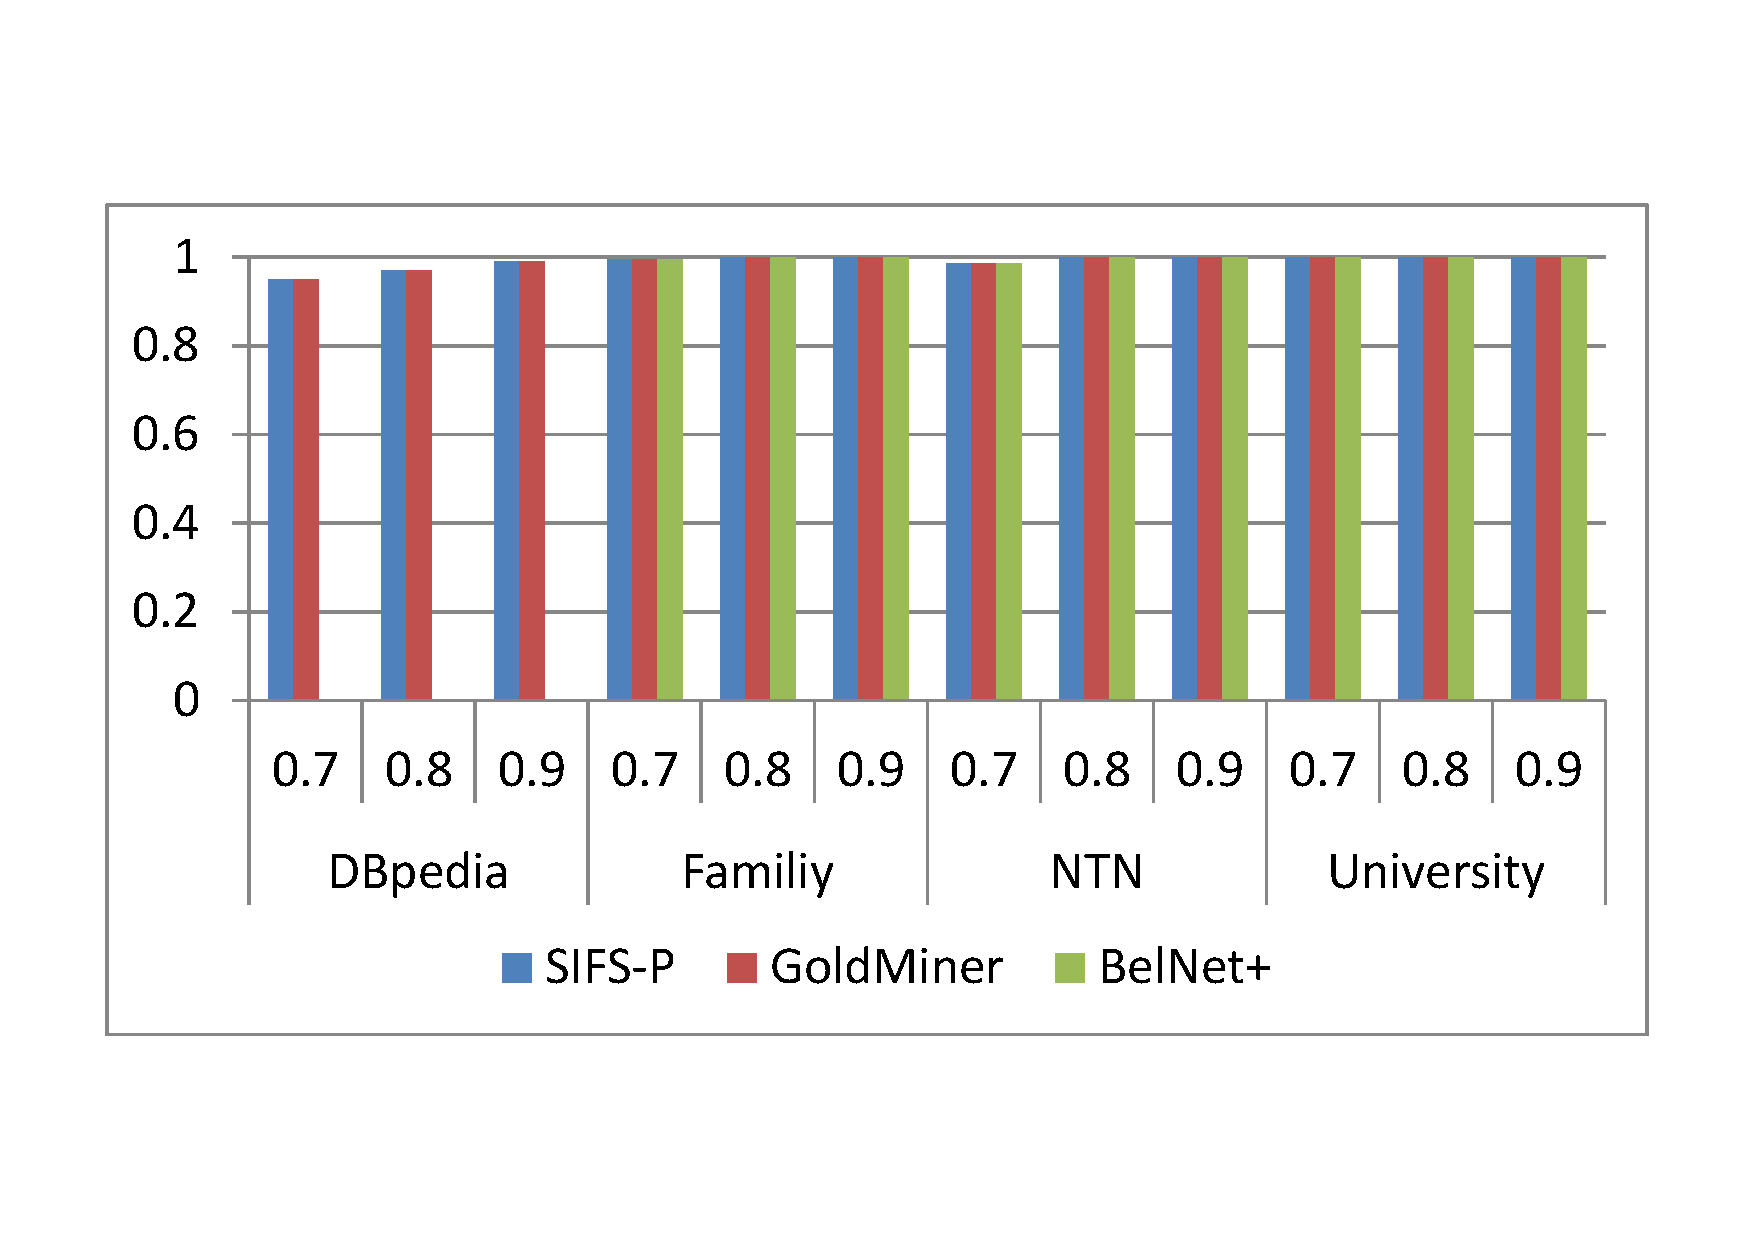
\includegraphics[width=0.49\textwidth]{figs/precision-subc.pdf}
  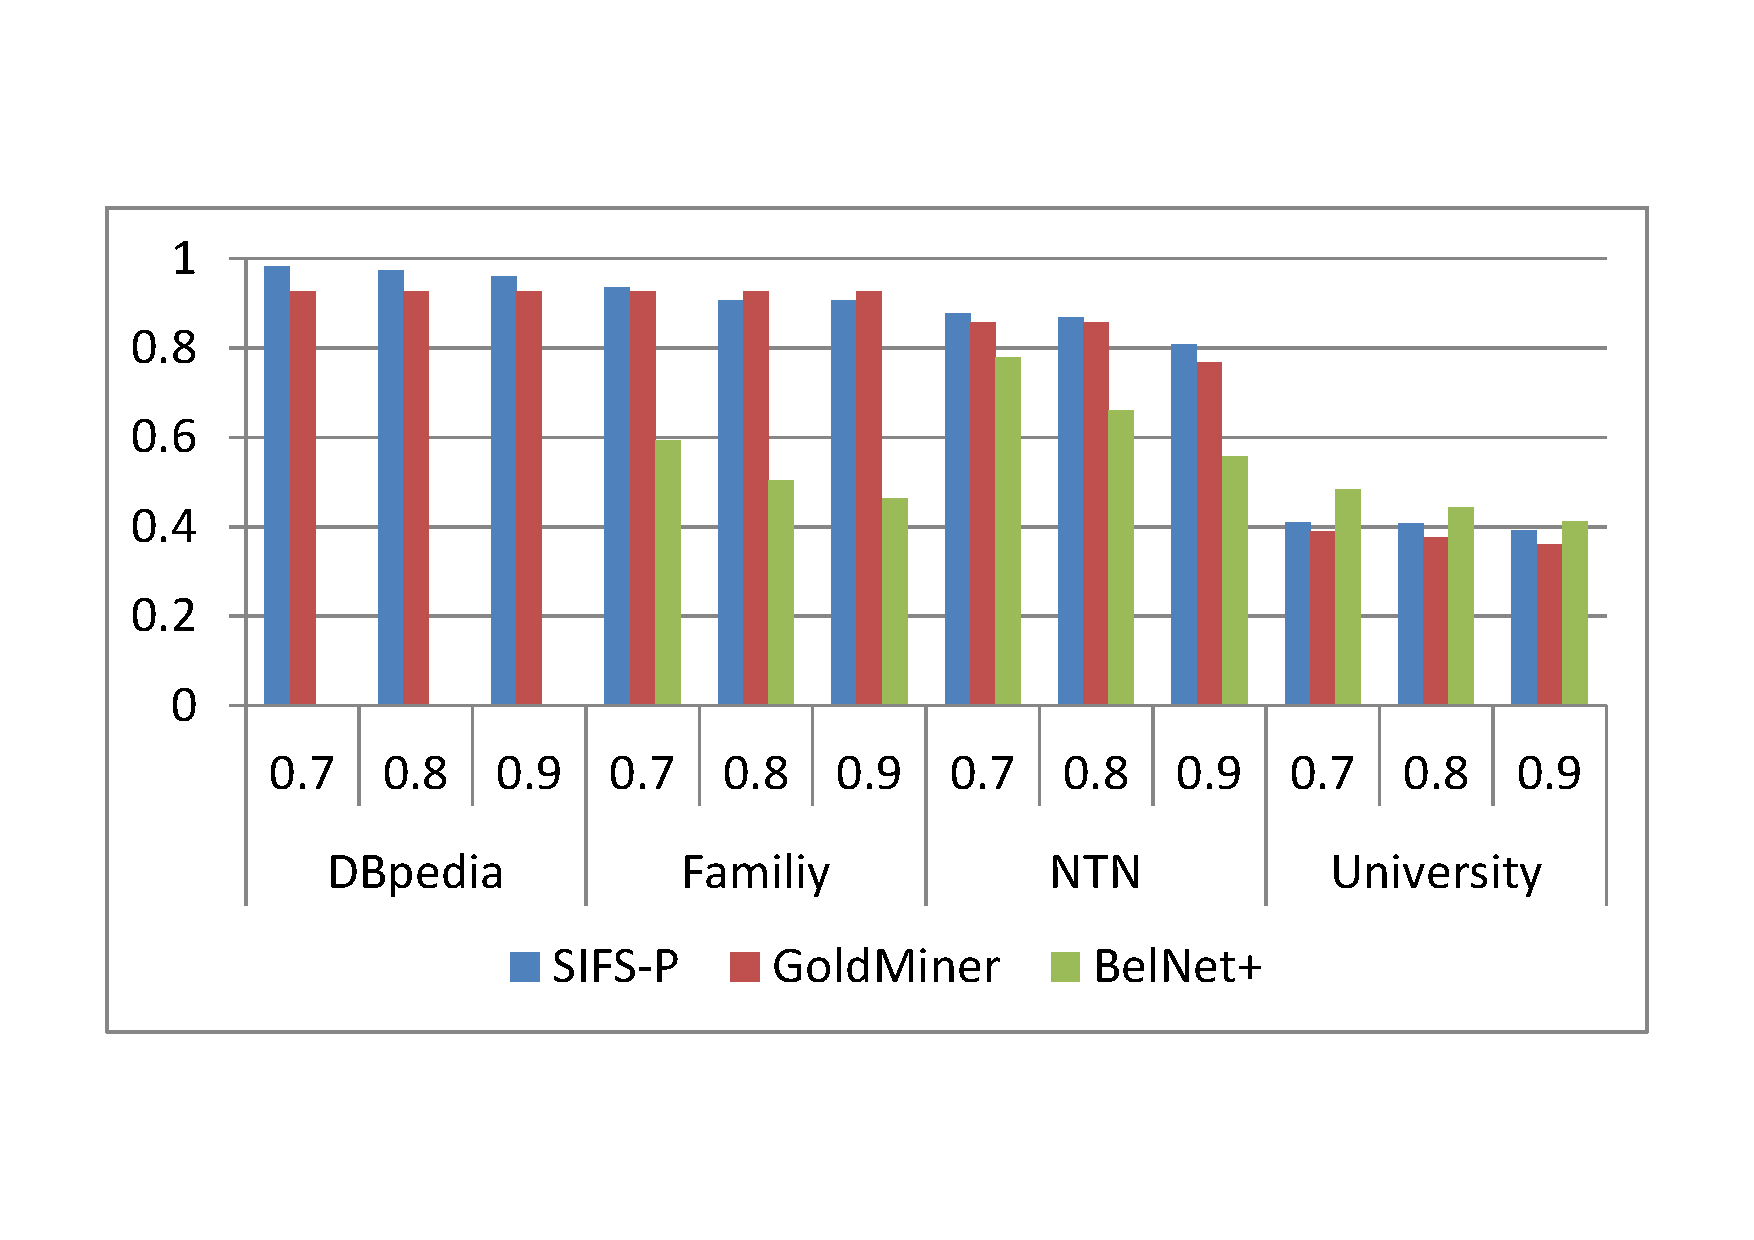
\includegraphics[width=0.49\textwidth]{figs/recall-subc.pdf}
  \caption{Precision (left) and recall (right) of systems to generate subclass axioms}\label{fig:precision-recall-subc}
\end{figure*}
\begin{figure*}
  \centering
  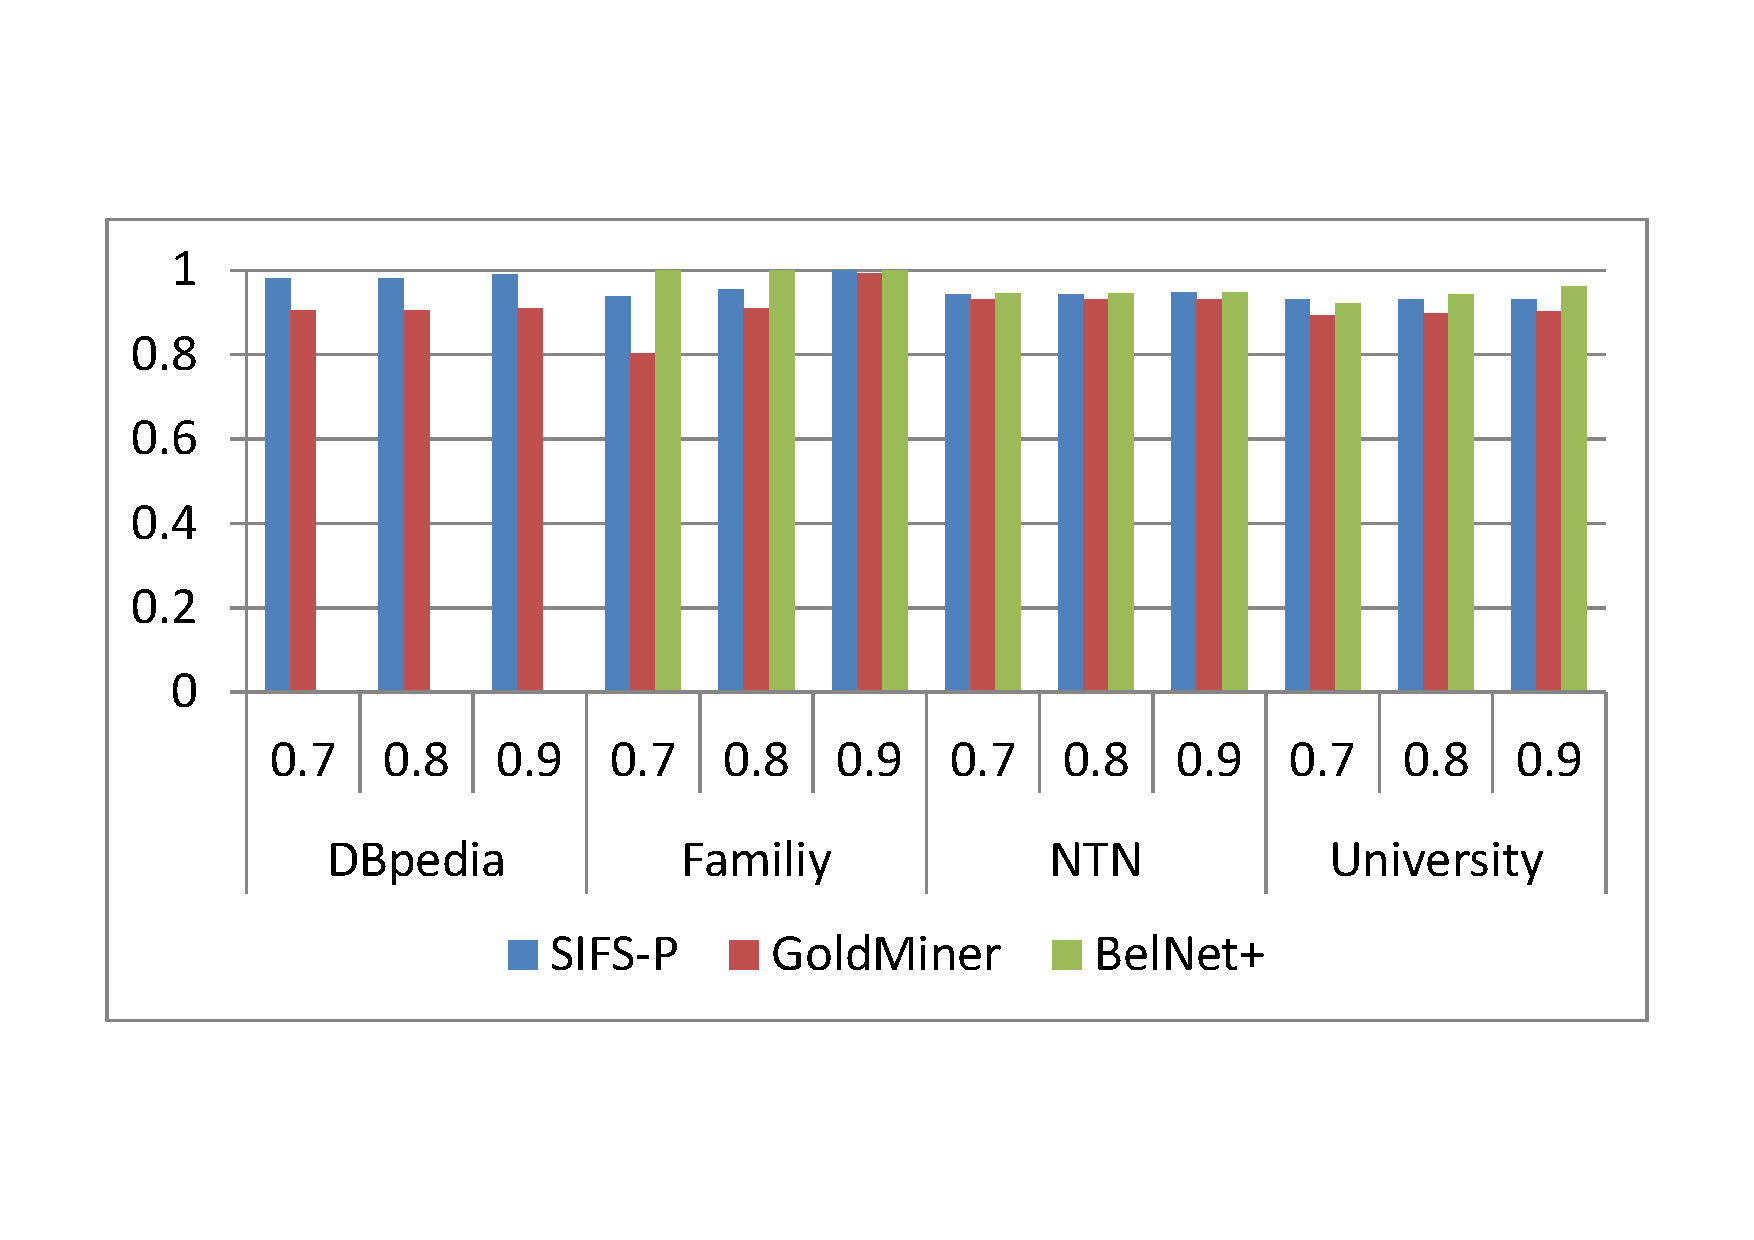
\includegraphics[width=0.49\textwidth]{figs/precision-disj.pdf}
  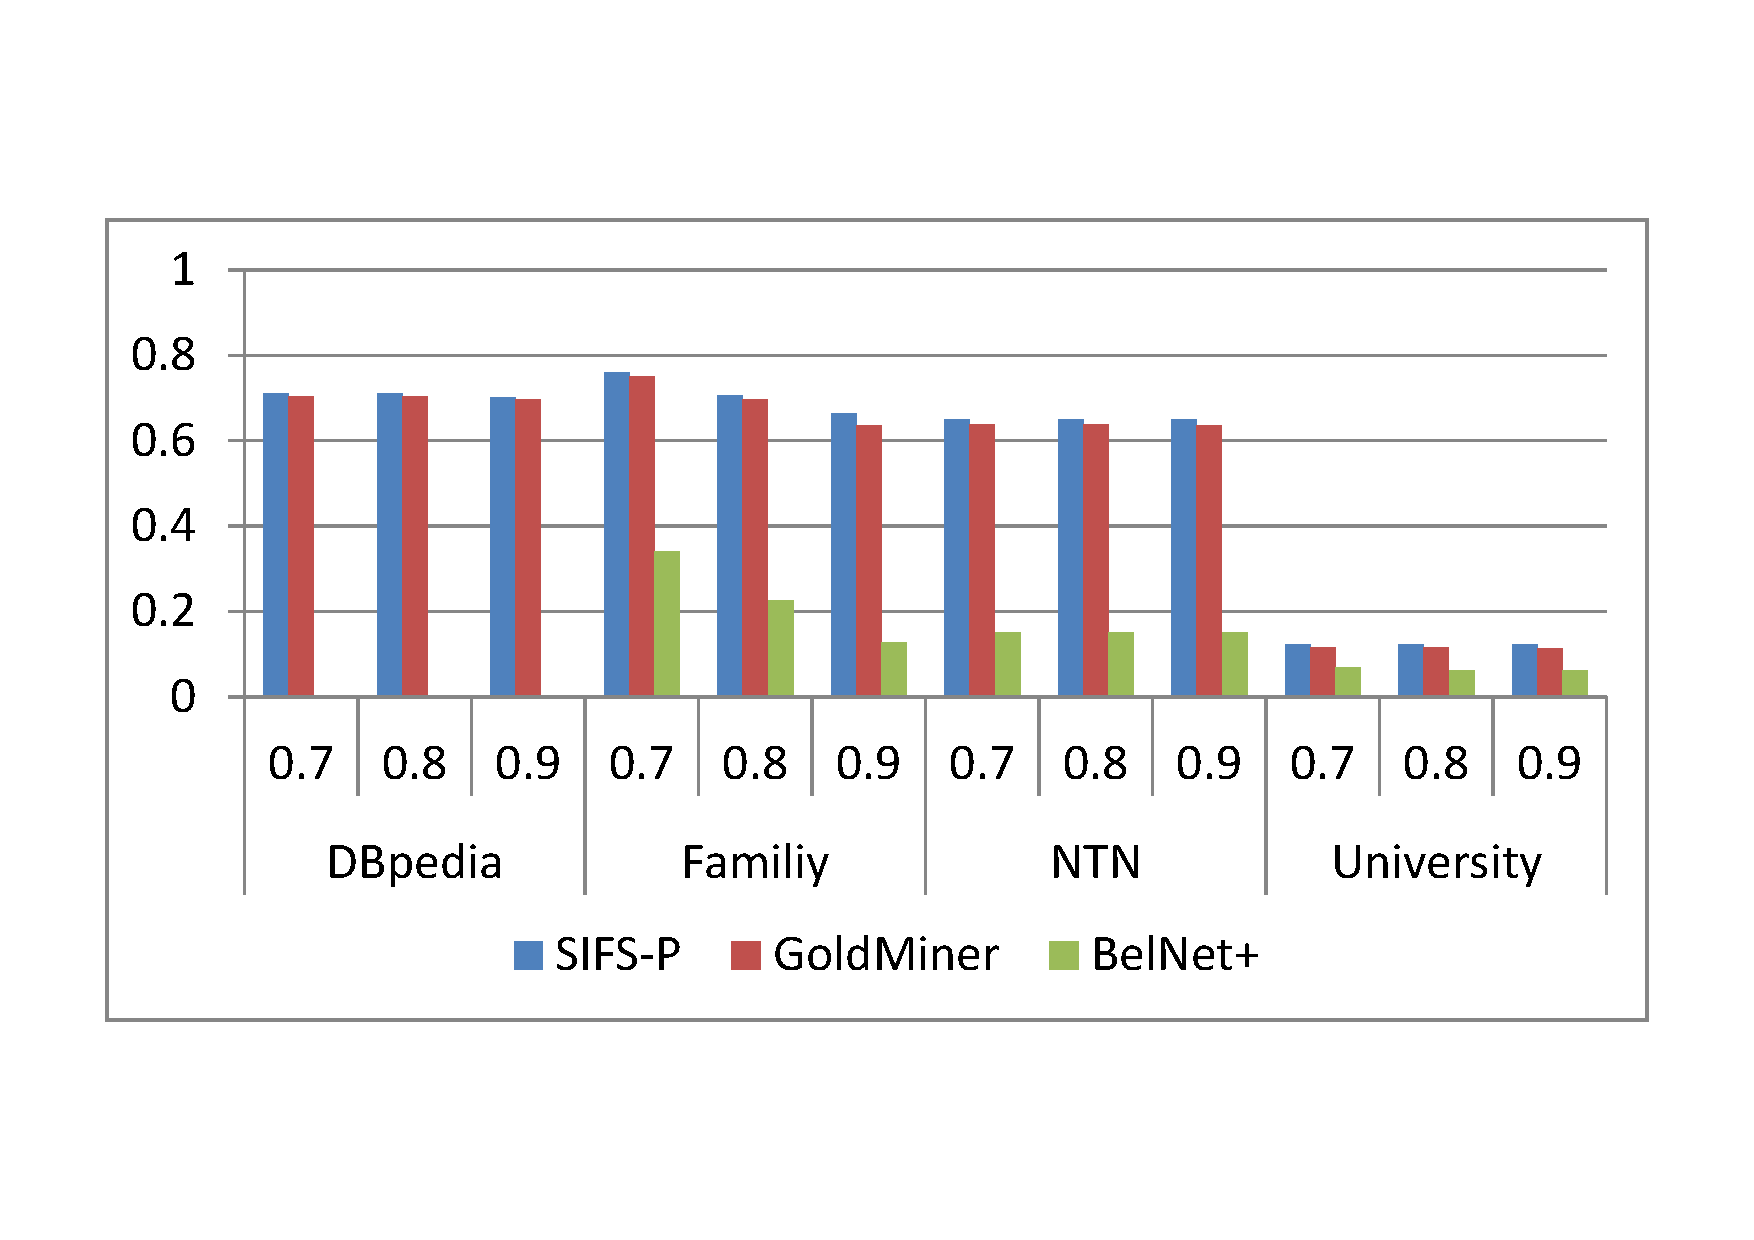
\includegraphics[width=0.49\textwidth]{figs/recall-disj.pdf}
  \caption{Precision (left) and recall (right) of systems to generate disjointness axioms}\label{fig:precision-recall-disj}
\end{figure*}

In our experiments, we compare our system SIFS-P using proportional support, which is the implementation of Algorithm \ref{alg:miningAlg}, with two relevant systems GoldMiner and BelNet\textsuperscript{+}. The precision and recall of the systems to generate subclass and disjointness axioms can be seen in Figure  \ref{fig:precision-recall-subc} and Figure \ref{fig:precision-recall-disj} respectively. In these figures, 0.7, 0.8 and 0.9 in the horizontal axis indicate the thresholds to filter those rules with lower confidences. Since BelNet\textsuperscript{+} fails to deal with large data like DBpedia, the comparison is conducted over other three KBs.

We first compare SIFS-P with GoldMiner. When mining subclass axioms, both systems have achieved very high precisions because almost all subclass axioms generated by them are correct. With respect to recall, SIFS-P performs better in most cases since more subclass axioms have been found by SIFS-P. This reflects the advantage of using type inference. That is, more type assertions recommended by type inference can increase the support of a rule and thus more correct subclass axioms could be generated.
%
When mining disjointness axioms, the advantage of using type inference becomes more obvious, especially for DBpedia. When the recalls of SIFS-P and GoldMiner are quite similar, the precisions of SIFS-P are much better.

%Comparing with the precision and recall of systems to generate disjointness axioms, those to generate subclass axioms are higher, especially with respect to recall (see the left figures in Figure \ref{fig:precision-recall-subc} and  \ref{fig:precision-recall-disj}). This has shown that generating disjointness axioms is much more challenging than generating subclass axioms.


Comparing SIFS-P with BelNet\textsuperscript{+}, the precisions of BelNet\textsuperscript{+} are more than 0.9, but 72\% of its recalls are no more than 0.6. For SIFS-P, the precisions are similar to those of BelNet\textsuperscript{+} while 67\% of its recalls are more than 0.6. This shows that BelNet\textsuperscript{+} generates much less disjointness axioms than SIFS-P.
%
BelNet\textsuperscript{+} depends on the joint probability to learn disjointness axioms. In the training stage, the number of individuals belonging to the pair of concepts is not large enough, which causes that many disjointness axioms are discarded when constructing the network.
%
The experimental results show again that SIFS-P could learn more disjointness axioms whose quality is also high due to the adoption of type inference.

